%!TEX root = ../Thesis.tex
\section{Beschreibung des Projektverlaufs}

\subsection{Tatsächliche Aufgabenverteilung im Team (tabellarisch)}

\subsection{Teammeeting-Protokolle}

 \para{03.09.2019 :: 200 Minuten}

\begin{itemize}
	\item Auswahl des Projekttyps. Das Team hat sich für die Entwicklung einer Android  App entschieden.
	\item Erste Einarbeitung in die Thematik. Lesen des bereitgestellten Dokuments mit Aufgabenstellung, groben Anforderungen und weiteres.
	\item Konzepterarbeitung auf Papier. Vorstellung und Diskussion verschiedener Ansätze.
\end{itemize}

\para{04.09.2019 :: 110 Minuten}

\begin{itemize}
	\item Sich mit Herr Seifert auf einen Ansatz für den Taschenrechner einigen.
	\item Workflow für Git, Meeting-Protokolle, Studienarbeit und Projekttagebücher festlegen.
	\item Ausarbeitung des Konzepts für den Taschenrechner. Hier wurden dem Auftraggeber Herr Seifert mehrere Konzepte vorgestellt und gemeinsam mit ihm genaue Anforderungen erarbeitet.
\end{itemize}

\para{05.09.2019 :: 20 Minuten}

Besprechen der Tagesziele:

\begin{itemize}
	\item Fertigstellung des Konzeptes.
	\item Fortschritte beim Paper-Prototypen machen bzw. erstellt haben.
	\item Android-Umgebung soll bei allen Team-Mitgliedern komplett aufgesetzt und lauffähig sein.
\end{itemize}

\para{05.09.2019 :: 60 Minuten}

Besprechen aktueller Stand des Konzepts und Prototypen:

\begin{itemize}
	\item Es wurde ein Mid-Fidelity Prototyp erstellt. 
	\item Diskussion über Umsetzung und Workflow der App.
	\begin{itemize}
		\item Wie sollen die einzelnen Kacheln funktionieren?
		\item Wie sollen die Kacheln miteinander interagieren?
		\item Wie könnte die Architektur der App aussehen?
	\end{itemize}
\end{itemize}

\para{05.09.2019 :: 40 Minuten}

\begin{itemize}
	\item Aufbau des Scrumboards mit Backlog, Doing, Review und Done.
	\begin{itemize}
		\item Backlog: Architektur Basics, Konzept (Paper Prototype, Mid-Fidelity-PPT-Prototyp), Rechenmodule, Zeitmanagement, UI-Coding-Design.
		\item Doing: Paper Mid Fidelity
		\item Review:
		\item Done: Git Projekt aufsetzen
	\end{itemize}
	\item Übertragen in Teams Planner und dort weitere Ausarbeitung.
	\item Grobe Verteilung der Einträge im Backlog um Konzepte zu erarbeiten.
\end{itemize}

\para{17.09.2019 :: 150 Minuten}

Backend-Architektur und App-Workflow:

\begin{itemize}
	\item Erweiterung UML-Klassendiagramm. Die Klasse Operand wird abstrakt und wird von konkreten Operanden wie Vector geerbt. Diese stellen Extensions dar die neben den eigentlichen mathematischen Werten weitere Daten und Verhalten mitbringen.
	\item Welche Library soll für Mathe-Funktionalitäten benutzt werden? JScience und die bereits mitgelieferte Standardbibliothek.
	\item Wie sollen Elemente in der GUI dargestellt werden? Als ASCII oder gerendert in LaTeX. Letzteres ist mit höherer Komplexität verbunden sieht aber auch besser aus. 
	\item Wie soll das Layout funktionieren? Gridlayout fällt raus, weil nicht dynamisch genug? Relative-Layout ist eine Option. Hier darf aber die Anordnung beim Rotieren nicht unkontrolliert verändert werden. UI Team möchte, dass alle Komponenten gleich groß sind. In dem Fall kann man Gridlayout benutzen.
	\item Wie soll die Eingabe von Funktionen im Graph Operand funktionieren? Nur möglich mit bereits vorhandenen Elementen in der Oberfläche. Es öffnet sich keine Tastatur.
\end{itemize}

\para{09.10.2019 :: 90 Minuten}

Verteilung von Programmieraufgaben und Diskussion:

\begin{itemize}
	\item Vorstellung des Backend-Entwurfs für Teammitglieder, die für das Frontend zuständig sind. 
	\item Vorstellung des Frontend-Entwurfs für Teammitglieder, die für das Backend zuständig sind.
	\item Diskussion über Verbindung von Frontend und Backend. Wie abgekoppelt lässt sich der Calculator wirklich realisieren?
	\item Vorstellung der Hauptbibliothek die für die (aufwändigen) Rechnungen wie Nullstellenberechnung benutzt werden soll.
	\item Warum Apache Commons Math und nicht JScience?
	\item Diskussion des Programm-Workflows.
	\item Diskussion ob ASCII-Darstellung oder LaTeX-Rendering für Frontend benutzt werden soll
\end{itemize}

\para{05.01.2020 :: 120 Minuten}

Arbeit am Projekt:

\begin{itemize}
	\item Aufnahme des aktuellen Projektstands.
	\item Besprechen des weiteren Vorgehens.
	\item Aufgabenabstimmung.
	\item Besprechung des geplanten Frontends.
	\item Besprechung/ Lösung von Problemen.
\end{itemize}

\para{14.01.2019 :: 90 Minuten}

Zusammenführung Frontend Backend:

\begin{itemize}
	\item Präsentation des Frontends durch das GUI-Team.
	\item Besprechen von MVC-Umsetzung in Android.
	\item Backend Unit-Testing Fortschritte.
	\item Serialisierung der Stacks zur Session-Sicherung.
\end{itemize}

\para{24.01.2019 :: 240 Minuten}

\begin{itemize}
	\item Detaillierte Ausarbeitung der Architektur im Backend.
	\item Programmieren im Team. 
	\item Zusammenführen mehrere Features.
	\item Umbau der Programmstruktur.
\end{itemize}

\para{28.01.2019 :: 90 Minuten}

Gespräch mit Herr Prof. Dr. Thomas Seifert über den aktuellen Stand des Projekts und im Anschluss daran eine Nachbesprechung innerhalb des Teams.

Vorstellung:

\begin{itemize}
	\item Vorstellung der bereits implementierten Grundfunktionen der App.
	\item Vorstellung des verwendeten Design-Patterns.
	\item Abgleich von Umsetzung mit den Anforderungen des Dozenten.
	\item Ansatz des Backends erklärt.
	\item Gerät ausleihen, um nicht nur mit Emulator testen zu können.
	\item Serialisierung der Daten (Speichern und Laden).
\end{itemize}

Ergebnis:

\begin{itemize}
	\item Projekt ist auf einem guten Weg. Priorisiert werden sollen differenzierende Funktionen anstatt wenige Features sehr detailliert auszuarbeiten (Prototypische Arbeit).
	\item Ternäre, Quaternäre usw. Operationen sind gewünscht.
	\item Vektoren in Bestandteile lösen.
	\item Eingabe von Matrizen.
	\item Jeder Klasse muss ein Verantwortlicher zugeordnet sein.
\end{itemize}

Ideen aus der Nachbesprechung:

\begin{itemize}
	\item ''Vektor bauen'' / ''Vektoren auflösen'' Action. 
	\item Summe von Stack Action.
	\item 1x Triple Operator einfügen.
	\item Operanden Eingabe via einzelne Menüs.
	\item Ranks der Stacks anpassen.
	\item Format des ersten Stacks anpassen (Format nicht 0,00).
\end{itemize}

\para{03.02.2019 :: 90 Minuten}

\begin{itemize}
	\item Besprechen des aktuellen Stands der App.
	\item Was muss noch unbedingt umgesetzt werden?
	\item Aufteilung der noch offenen Kapitel in der Ausarbeitung.
	\item Neues Kapitel ''Einleitung'' mit Motivation.
	\item Anpassung einiger Kapitelbezeichnungen an Gegebenheiten des Projekts.
\end{itemize}

\subsection{Projekttagebücher aller Teammitglieder (tabellarisch)}

\subsubsection{Tom Bockhorn}

\subsubsection{Hendrik Falk}

\subsubsection{Dennis Gentges}

\subsubsection{Getuart Istogu}

\subsubsection{Jannis Keienburg}

\subsubsection{Tim Jonas Meinerzhagen}

\subsubsection{Khang Pham}

\subsubsection{Tim Schwenke}

\subsection{Beschreibung von Problemen}

\subsubsection{Softwareentwicklung im Team [Schwenke]}

Schon kurz nach der initialen Erstellung des Git-Repositories und des Projekts in Android-Studio hat sich die Frage gestellt, wie man in einem acht Mitglieder starkem Team produktiv an einer einzelnen Code-Basis arbeiten soll. Hat man ein Quellcodeverzeichnis alleine für sich reichen zumeist um die drei aktive (also nicht \textit{stale}) Branches aus. Das wäre zunächst der \code{Master}-Branche, welcher die Wurzel des Verzeichnisses darstellt und – gerade, wenn Ansätze wie CI/CD verfolgt werden – die produktiven oder zumindest lauffähigen Versionen eines Projekts enthält. Im \code{Development}-Branch hingegen findet die Entwicklung statt. Hier ist es üblich, dass das Projekt zum Zeitpunkt einzelner Commits Fehler enthält und nicht lauffähig ist. Sobald ein Entwickler der Meinung ist, dass der Stand in \code{Development} veröffentlicht werden kann, wird \code{Development} in \code{Master} vereint. Wichtig zu betonen ist hier, dass dies keine feste Regel ist, sondern eher dem allgemeinen Workflow entspricht. In einem großen Team ist ein solcher Arbeitsablauf nicht mehr möglich. So müssen mehrere Entwickler parallel an dem Projekt arbeiten. Verwendet man nun das System aus zwei Branches, wird es sehr schnell zu Merge-Konflikten kommen, die die Entwickle dazu zwingen sich mehr mit der korrekten Zusammenführung als der eigentlichen Entwicklung zu beschäftigen, sofern sie ihren lokalen Arbeitsbereich aktuell halten wollen. Die nächstliegende und ebenfalls problematische Alternative ist es nur bei Fertigstellung von Funktionen, die meist aus mehreren Commits zusammengesetzt sind, das lokale Quellcodeverzeichnis mit dem Remote zu synchronisieren. Mit dieser Herangehensweise verpasst man unter Umständen große Fortschritte im Gesamtprojekt. Die lokale Version ist plötzlich nicht mehr lauffähig und muss aufwändig angepasst werden. Deswegen haben wir uns in diesem Projekt für den Gitflow-Workflow entschieden. Grafisch dargestellt ist dieser beispielhaft in der folgenden Grafik.

\begin{figure}[h]
	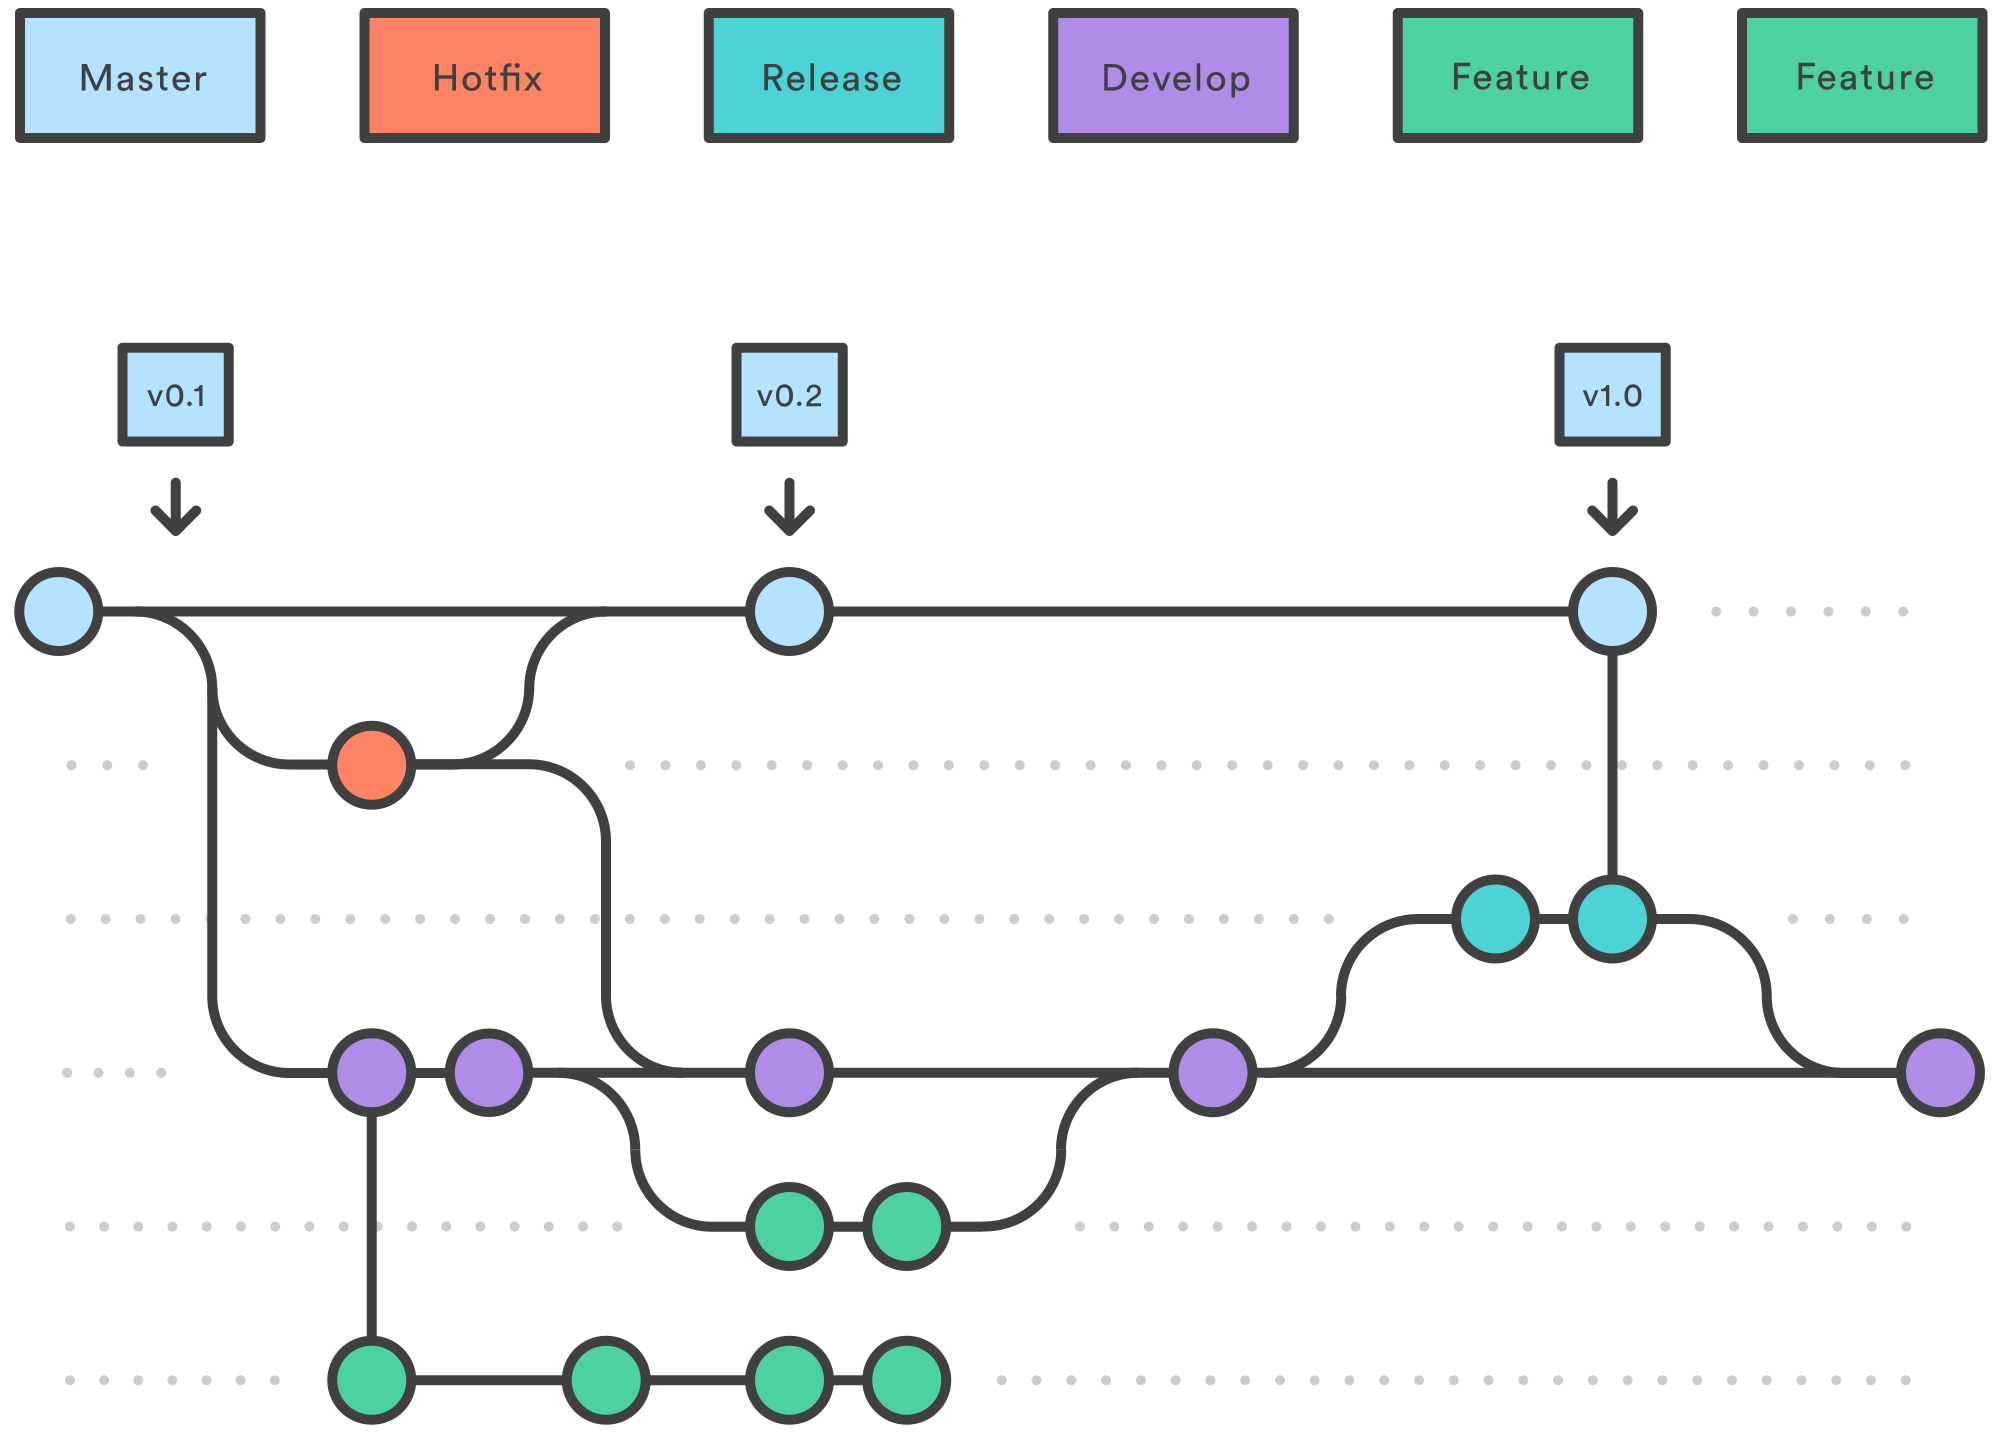
\includegraphics[width=\columnwidth]{img/gitflow}
	\caption[Gitflow]{Gitflow\footnotemark}
\end{figure}
\footnotetext{\cite{atlassian2020}}

Der Gitflow-Workflow definiert ein strenges Branching-Model und gibt jedem Typ von Branch (lediglich differenziert durch ihre Namen) eine spezifische Rolle. \code{Master} wird verwendet, um die Release-History festzuhalten. Hier finden sich Versionen des Projekts, die lauffähig sind und für sich alleine stehen (können). \code{Development} fungiert ähnlich wie \code{Master}, nur enthält es die gesamte Entwicklungshistorie des Projekts. Nun kommen die sogenannten \code{Feature}-Branches ins Spiel, die beliebig weiter untergliedert werden können. Benannt werden Features hierarchisch. In unserem Projekt haben wir folgende zwei Gruppen von Feature-Branches: 

\texttt{feature/backend/<konkretes-feature>}

\texttt{feature/frontend/<konkretes-feature>}

Jedes Feature wird einem Verantwortlichen zugeteilt und wird meist auch von diesem bearbeitet. Sobald ein Feature fertig ist, wird es in \code{Development} zusammengeführt. Somit werden die Abstände zwischen Zusammenführungen verringert und der Arbeitsablauf wird einfacher. Schließlich gibt es auch noch einen Hotfix-Branch, für dringende Änderungen.

Im Laufe der Entwicklung haben sich die Vorteile dieser Herangehensweise für das Team deutlich gezeigt. Unterschiedliche Features konnten, nachdem eine grundlegende Programmarchitektur umgesetzt wurde, meist ohne Probleme zusammengeführt werden. 